\documentclass[12pt]{article}

% Packages
\usepackage[utf8]{inputenc}
\usepackage[T1]{fontenc}
\usepackage{lipsum} % For generating dummy text
\usepackage[margin=2cm]{geometry} % Adjust the margin size here
\usepackage{amsmath}
\usepackage{graphicx}
\usepackage{mdframed}

% my formulae
\newcommand{\bold}[1]{\textbf{#1}}



% Title and author
\title{NLP CS5803 IITH Notes}
\author{Deepak}

\begin{document}

\maketitle
\tableofcontents

\newpage

\section{Introduction}
The starting question is how to make computers understand human
language. We need to find smart ways of representing the language.

\section{Input Representation}
    Consider text modality, where the input is a document, it
    consists of words(also called tokens). The document is represented
    by the set of words/tokens it contains.

    Lets see some methods for text representation
    

    \subsection{TF-IDF scheme}

        \subsubsection{Formulation}
            The TF-IDF (Term Frequency-Inverse Document Frequency) scheme is a
            popular technique used to represent the importance of words in a 
            document corpus. \\
            It combines two factors: term frequency (TF) and inverse document frequency (IDF). \\
            \bold{TF} measures the frequency of a term in a document. 
            It is calculated by counting the number of occurrences of a term 
            in a document as a raw or by taking a log of it.

            \[
            \text{tf}(t, d) = \begin{cases}
                            0 & \text{if } c(t, d) = 0 \\
                            1 + \log(c(t, d)) & \text{if } c(t, d) \neq 0
                        \end{cases}
            \]

            where $c(t, d)$ is the count of term $t$ in document $d$.
            \\
            \bold{IDF} de-emphasizes the frequent words across the corpus
            (all documents combined is usually called corpus) and emphasizes
            the on words differentiating the documents.

            \[
            \text{idf}(t) = \log_{10} \left( \frac{N}{\text{df}_{t}}\right)
            \]
            
            where $N$ is the total number of documents in the corpus and $\text{df}_{t}$ is the number of documents containing the term $t$.
            \\
            The TF-IDF score for a term in a document is obtained by multiplying its TF value with its IDF value. Mathematically, it can be represented as:

            \[
            \text{tf-idf}(t, d) = \text{tf}(t, d) \times \text{idf}(t)
            \]
            Now we get a table with TF-IDF values.
            
            This way, each document is represented by a vector from the column
            of the table and each word is presented by a vector from
            the row of the table.

            \subsubsection{Limitation}
            \begin{itemize}
                \item Words are considered at their lexical appearance
                \item Synonymy is not considered
                \item Polysemy(word with multiple meanings) is not considered
                \item long sparse vectors
                \item context is not considered
            \end{itemize}

    \subsection{SVD - text representation}
        \subsubsection{Formulation}
            Consider the term-document matrix and apply SVD to it
            to do dimensionality reduction, so that we can get dense
            representations.
            \\
            Let A be the term-document matrix(matrix with freq. of words in docs), 
            where each row represents a term and each column represents a document, 
            by SVD we have

            \[
                A = U \Sigma V^{T}
            \]
            U, V are orthonormal matrices and $\Sigma$ is a diagonal matrix of 
            singular values of A in decreasing order.
            \\
            By keep only the first k singular values, we have

            \[
                A_k = U_k \Sigma_k V_k^{T}
            \]

            The k here is much smaller than the original dimension of A.
            Terms can be represented by the rows of $U_k$ and documents can be
            represented by the columns of $V_k$.
            
    \subsection{LDA - text representation}
        \subsubsection{Formulation}
            LDA (Latent Dirichlet Allocation) is a text representation based
            on \bold{topics}. It assumes that each document is a mixture of 
            topics which are latent or unknown. Words in a document depend on
            topics of the document. LDA is a mechanism to identify the topics
            and connect words with topics
            \\
            The generative process is as follows:
            \begin{itemize}
                \item For each document, draw a distribution over topics
                \item For each word in the document, draw a topic from the
                distribution over topics and then draw a word from the
                distribution over words for that topic.
            \end{itemize}
            The parameters of the model are the topic distributions for each
            document, the word distributions for each topic, and the topic
            distribution over the entire corpus.
            \\
            The model is trained by maximizing the likelihood of the observed
            documents. The topic distributions for each document and the word
            distributions for each topic are learned from the data.
            \\
            The learned topic distributions for each document can be used to
            represent the documents and the learned word distributions for each
            topic can be used to represent the topics.
            
        \subsubsection{Mathematical Formulation}

            The mathematical formulation of LDA is as follows:
            
            For each document $d$ in the corpus $D$:
            
            1. Choose $N \sim Poisson(\xi)$.
            
            2. Choose $\theta \sim Dir(\alpha)$.
            
            3. For each of the $N$ words $w$:
            
                a. Choose a topic $z \sim Multinomial(\theta)$.
            
                b. Choose a word $w$ from $p(w|z,\beta)$, a multinomial probability conditioned on the topic $z$.
            
            Here, $\xi$ is the parameter of the Poisson distribution used to choose the number of words in a document, $\alpha$ is the parameter of the Dirichlet distribution used to generate the per-document topic distributions, and $\beta$ is the parameter of the multinomial distribution used to generate the per-topic word distribution.
        

    \subsection{Word2Vec}
        \bold{Context of words}: Context of a word is the set of words that surround it.
        For example, in the sentence "I love to eat pizza", the context of the word "love" is \{"I", "to", "eat"\}.
        \\
        Note: Word2Vec models rely on "distributional symmetry" hypothesis, i.e. similar words have similar contexts.
        \\
        Word2Vec is a popular technique used to represent words in a continuous vector space. \\
        It is based on the idea that words that appear in similar contexts are semantically similar.
        Word2Vec has two models: SkipGram and Continuous Bag of Words (CBOW).
        \begin{figure}[h]
            \centering
            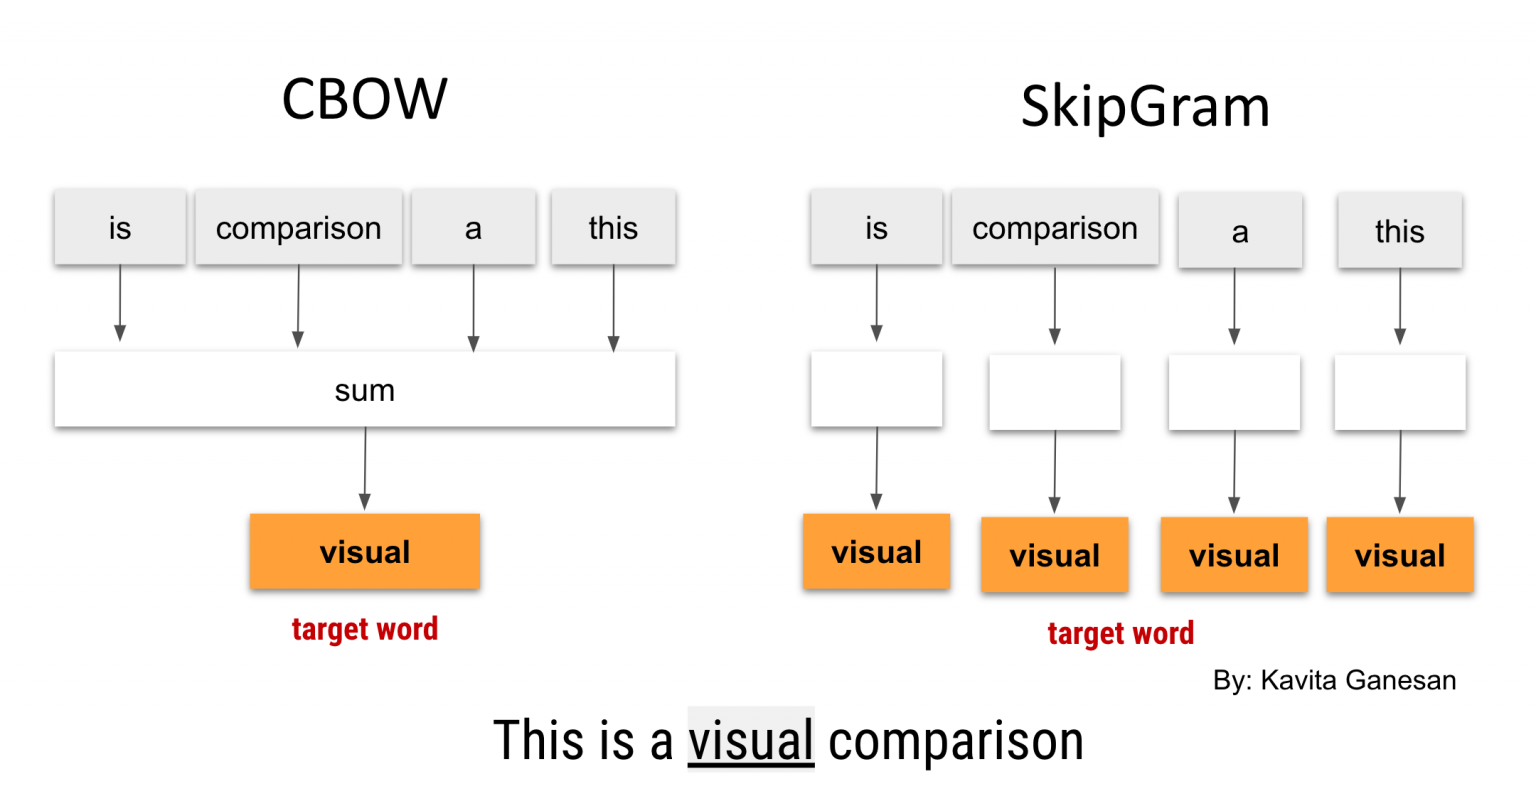
\includegraphics[width=0.5\textwidth]{/workspaces/DartBase/notes/nlp/images/cbow_vs_sg.png}
        \end{figure}
        \subsubsection{Continuous Bag of Words (CBOW)}
            This model predicts the middle word based on the context words.
            
            We create two matrices, $V \in \bold{R}^{n \times |V|}$ and $U \in \bold{R}^{|V| \times n}$. Where $n$ is an arbitrary size which defines the size of our embedding space.
            \begin{mdframed}
            $w_i$: Word $i$ from vocabulary $V$ \\
            $V \in \bold{R}^{n \times |V|}$: Input word matrix \\
            $v_i$: $i_{th}$ column of $V$, the input vector representation of word $w_i$\\
            $U \in \bold{R}^{n \times |V|}$: Output word matrix\\
            $u_i$: $i_{th}$ row of $U$, the output vector representation of word $w_i$
            \end{mdframed}
            Note that we do in fact learn two vectors for every word $w_i$ (i.e. input word vector $v_i$ and output word vector $u_i$).
            \begin{figure}[h]
                \centering
                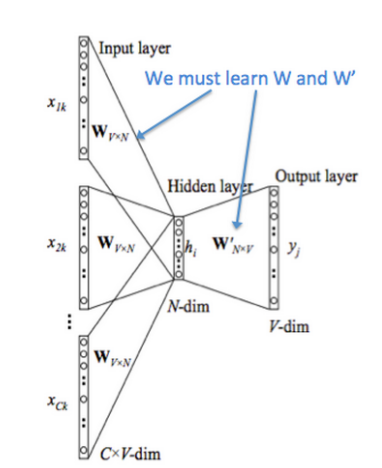
\includegraphics[width=0.5\textwidth]{/workspaces/DartBase/notes/nlp/images/cbow_net.png}
            \end{figure}
            also, the below steps are done using a single hidden layer neural network.\\
            We breakdown the way this model works in these steps:
            \begin{enumerate}
                \item We generate our one hot word vectors $(x_{c-m}, \ldots, x_{c-1}, x_{c+1}, \ldots, x_{c+m})$ for the input context of size $m$.
                \item We get our embedded word vectors for the context  \\
                $(v_{c-m} = Vx_{c-m}, v_{c-m+1} = Vx_{c-m+1}, \ldots, v_{c+m} = Vx_{c+m})$.
                \item Average these vectors to get $\hat{v} = \frac{v_{c-m} + v_{c-m+1} + \ldots + v_{c+m}}{2m}$.
                \item Generate a score vector $z = U\hat{v}$.
                \item Turn the scores into probabilities $\hat{y} = \text{softmax}(z)$.
                \item We desire our probabilities generated, $\hat{y}$, to match the true probabilities, $y$, which also happens to be the one hot vector of the actual word.
            \end{enumerate}
            
            Since, we have a neural network we need objective function.
            we use a popular choice of distance/loss
            measure, cross entropy $H(\hat{y}, y)$.

            \begin{align*}
                H(\hat{y}, y) &= -\sum_{i=1}^{|V|} y_i \log(\hat{y}_i) \\
                &= -\log(\hat{y}_j)\\
                &= - \log \frac{\exp(z_c)}{\sum_{j=1}^{|V|} \exp(z_j)} \\
                &= - \log \frac{\exp(u_c^T \hat{v})}{\sum_{j=1}^{|V|} \exp(u_j^T \hat{v})} \\
                &= - \log P(u_c|\hat{v}) \\
                &= - \log P(w_c|w_{c-m}, \ldots, w_{c-1}, w_{c+1}, \ldots, w_{c+m})
            \end{align*}
            
            Hence, it perfectly makes sense to choose the cross entropy as our loss function.
        
        \subsubsection{SkipGram}
            Predicting surrounding context words given the middle word.\\
            \begin{figure}[h]
                \centering
                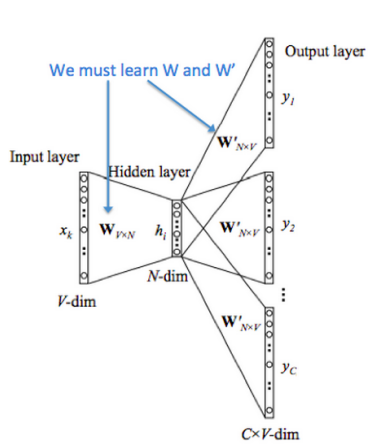
\includegraphics[width=0.5\textwidth]{/workspaces/DartBase/notes/nlp/images/sg_net.png}
            \end{figure}
            
            The setup is largely the same but we essentially swap our $x$ and $y$ i.e. $x$ in the CBOW are now \\ $y$ and vice-versa. 
            The input one hot vector (center word) we will represent with an $x$ (since there is only one). 
            And the output vectors as $y^{(j)}$. We define $V$ and $U$ the same as in CBOW.


            We breakdown the way this model works in these 6 steps:
            \begin{enumerate}
                \item We generate our one hot input vector $x$.
                \item We get our embedded word vectors for the context $v_c = Vx$.
                \item Since there is no averaging, just set $\hat{v} = v_c$.
                \item Generate $2m$ score vectors, $u_{c-m}, \ldots, u_{c-1}, u_{c+1}, \ldots, u_{c+m}$ using $u = Uv_c$.
                \item Turn each of the scores into probabilities, $\hat{y} = \text{softmax}(u)$.
                \item We desire our probability vector generated to match the true probabilities which is \\
                 $y_{c-m}, \ldots, y_{c-1}, y_{c+1}, \ldots, y_{c+m}$, the one hot vectors of the actual output.
            \end{enumerate}
            
            As in CBOW, we need to generate an objective function for us to
            evaluate the model. A key difference here is that we invoke a Naive
            Bayes assumption to break out the probabilities
            \begin{align*}
                J &= - \log P(w_{c-m}, \ldots, w_{c-1}, w_{c+1}, \ldots, w_{c+m}|w_c) \\
                &= - \log \prod_{j=0, j \neq m}^{2m} P(w_{c-m+j}|w_c) \\
                &= - \log \prod_{j=0, j \neq m}^{2m} P(u_{c-m+j}|v_c) \\
                &= - \log \prod_{j=0, j \neq m}^{2m} \frac{\exp(u_{c-m+j}^T v_c)}{\sum_{k=1}^{|V|} \exp(u_k^T v_c)} \\
                &= - \sum_{j=0, j \neq m}^{2m} u_{c-m+j}^T v_c + 2m \log \sum_{k=1}^{|V|} \exp(u_k^T v_c)
            \end{align*}

            Similar to CBOW this can also be written as error between $y^i$ and $\hat{y^i}$ .
        \subsubsection{Negative Sampling}
        Note that the
        summation over |V| is computationally huge! Any update we do or
        evaluation of the objective function would take O(|V|) time which
        if we recall is in the millions. This is where negative sampling comes
        to the rescue. The idea is to sample a small number of negative
        examples (words that are not in the context of the center word).

        While negative sampling is based on the Skip-Gram
        model, it is in fact optimizing a different objective.

        Consider a pair $(w, c)$ of word and context word.
        Let's denote by $P(D = 1|w, c)$ the probability that $(w, c)$ came from the corpus data. Correspondingly, $P(D = 0|w, c)$ will be the
        probability that $(w, c)$ did not come from the corpus data. First, let's model $P(D = 1|w, c)$ with the sigmoid function:
        \[P(D = 1|w, c, \theta) = \frac{1}{1 + e^{-v_c^T v_w}}\]
         
        Now, we build a new objective function that tries to maximize the probability of a word and context being in the corpus data if it indeed is, and maximize the probability of a word and context not being in the corpus data if it indeed is not. We take a simple maximum likelihood approach of these two probabilities. (Here we take $\theta$ to be the parameters of the model, and in our case it is $V$ and $U$.)

        \begin{align*}
            \theta &= \arg\max_{\theta} \prod_{(w,c) \in D} P(D = 1|w, c, \theta) \prod_{(w,c) \in \tilde{D}} P(D = 0|w, c, \theta) \\
            &= \arg\max_{\theta} \prod_{(w,c) \in D} P(D = 1|w, c, \theta) \prod_{(w,c) \in \tilde{D}} (1 - P(D = 1|w, c, \theta)) \\
            &= \arg\max_{\theta} \sum_{(w,c) \in D} \log P(D = 1|w, c, \theta) + \sum_{(w,c) \in \tilde{D}} \log(1 - P(D = 1|w, c, \theta)) \\
            &= \arg\max_{\theta} \sum_{(w,c) \in D} \log \frac{1}{1 + \exp(-u_w^T v_c)} + \sum_{(w,c) \in \tilde{D}} \log\left(1 - \frac{1}{1 + \exp(-u_w^T v_c)}\right) \\
            &= \arg\max_{\theta} \sum_{(w,c) \in D} \log \frac{1}{1 + \exp(-u_w^T v_c)} + \sum_{(w,c) \in \tilde{D}} \log\left(\frac{1}{1 + \exp(u_w^T v_c)}\right)
        \end{align*}
        This changes as follows by considering k negative samples for each postive.
        \[
            \log \sigma(u_{c-m+j}^T v_c) + \sum_{k=1}^{K} \log \sigma(-\tilde{u}_k^T v_c)
        \]
        In the above formulation, $\{\tilde{u}_k | k = 1, \ldots, K\}$ are sampled from $P_n(w)$.
        the n value of 0.75 seems work well in practice, since it increase the high probability words 
        less, while low probability words more.

    \subsection{GloVe}
        Emphasizes on co-occurrence with context/ Probe word 
        \begin{mdframed}
            Co-occurrence Matrix:
            \begin{itemize}
                \item $X$: word-word co-occurrence matrix
                \item $X_{ij}$: number of times word $j$ occur in the context of word $i$
                \item $X_i = \sum_k X_{ik}$: the number of times any word $k$ appears in the context of word $i$
                \item $P_{ij} = P(w_j | w_i) = \frac{X_{ij}}{X_i}$: the probability of $j$ appearing in the context of word $i$
            \end{itemize}
        \end{mdframed}

        Focus on ratio of co-occurrence probabilities
        Given words $w_i$, $w_j$, and $w_k$, the ratio of their co-occurrence probabilities is:
        \[
            F(w_i, w_j, \tilde{w}_k) = \frac{P_{ik}}{P_{jk}}
        \]
        Word embeddings are linear in structures
        so, the natural way of defining F is using subtraction and multiplication
        \[
            F((w_i-w_j)^T\tilde{w}_k) = \frac{P_{ik}}{P_{jk}}
        \]
        , the distinction between a word and a context word is arbitrary and that we are free to 
        exchange the two roles. To do so consistently, we must not only exchange $w \leftrightarrow 
        \tilde{w}$ but also $X \leftrightarrow X^T$. Our final model should be invariant under this relabeling.
        
        However, the symmetry can be restored in two steps. \\
        First, we require that $F$ be a 
        homomorphism between the groups $(\bold{R},+)$ and $(\bold{R}_{>0}, \times)$, i.e.,
        
        \[
            F((w_i - w_j)^T \tilde{w}_k) = \frac{F(w_i^T \tilde{w}_k)}{ F(w_j^T \tilde{w}_k)}
        \]

        which implies $F(w_i^T \tilde{w}_k) = P_{ik} = \frac{X_{ik}}{X_i}$. \\
        then $F = \exp$, or, $w_i^T \tilde{w}_k = \log(P_{ik}) = \log(X_{ik}) - \log(X_i)$

        We can observe the equation becomes symmetric if not for $log(X_i)$.
        This term is independent of $k$ so it can be absorbed into a bias $b_i$ for $w_i$. Finally, adding an additional bias $\tilde{b}_k$ for $\tilde{w}_k$ restores the symmetry,
        \[w_i^T \tilde{w}_k + b_i + \tilde{b}_k = \log(X_{ik}).\]

        Need to weigh all co-occurrences differently, as some words
        that happen to occur rarely or never. 

        Proposed a new weighted least squares regression model that addresses these problems.
        \[
            J = \sum_{i,j=1}^{V} f(X_{ij}) (w_i^T \tilde{w}_j + b_i + \tilde{b}_j - \log X_{ij})^2
        \]
\end{document}
